\section{Thread in OS161}



\begin{center}
  \begin{minipage}{0.65\linewidth}

    Il kernel ha bisogno di due tipologie di thread:
    \textbf{user thread} - utilizzate dalle librerie utente -  e \textbf{kernel thread} -
    supportate del kernel.
  \end{minipage}%
  \hfill
  \begin{minipage}{0.3\linewidth}
    \centering
    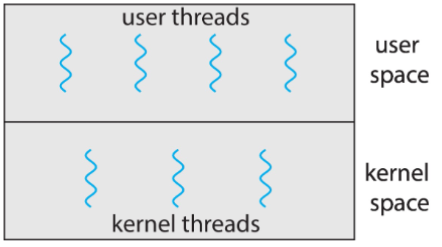
\includegraphics[width=\linewidth]{content/OS_Internals/images/2026-05-05-13-32-16.png}
  \end{minipage}
\end{center}




\begin{center}
  \begin{minipage}{0.5\linewidth}
    Un \textbf{Thread} rappresenta il control state di un processo (programma in eseguzione).
    Questo context include:
    \begin{itemize}
      \item lo stato del processore come registri, SP, etc;
      \item Stack, localizzato nell'address space del processo
    \end{itemize}

    I thread possono essere many-to-one, one-to-one o many-to-many.

    La memoria, come sappiamo già, contiene il codice, i dati e lo stack che contiene il
    record di attivazione delle funzioni.
  \end{minipage}%
  \hfill
  \begin{minipage}{0.\linewidth}
    \centering
    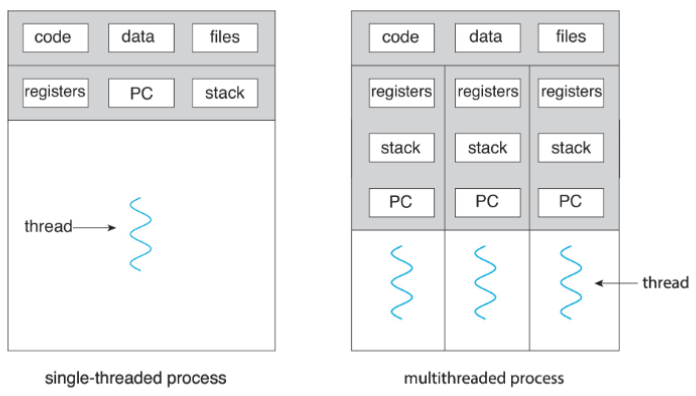
\includegraphics[width=\linewidth]{content/OS_Internals/images/2026-05-05-13-34-37.png}
  \end{minipage}
\end{center}

\textbf{Switch frame}, usato in OS161 per il context switch - running, ready, blocked etc.
\textbf{Trap frame}, usato per gestire le interruzioni - simile al ritorno da una funzione.



\section{Memoria in OS161}


\begin{center}
  \begin{minipage}{0.75\linewidth}
    La memoria ha un indirizzo fisico e uno virtuale, in OS161 usa sempre la TLB, anche se non
    c'è la page table. Se da TLB miss chiama la gestione di un page fault. Se c'è allocazione
    continua come in DUMBVM è un misto tra allocazione contigua e usa la TLB.

    I primi due inidirizzi logici sono per user e gli altri due per kernel, così
    basta guardare l'indirizzo per capire se è user o kernel.

    MIPS se l'indirizzo è minore di 2GB uso la TLB, altriment: kseg0 usa relocation
    pensa il processore (aggiungendo 2GB), kseg1 stanno i dispositivi IO mapped in memory e \textbf{non}
    usa la cache (perché io voglio scrivere ma non rileggere quello che ho scritto ma l'effetto),
    kseg2 alcune strutture del kernel che possono essere paginate (non usato).

  \end{minipage}%
  \hfill
  \begin{minipage}{0.2\linewidth}
    \centering
    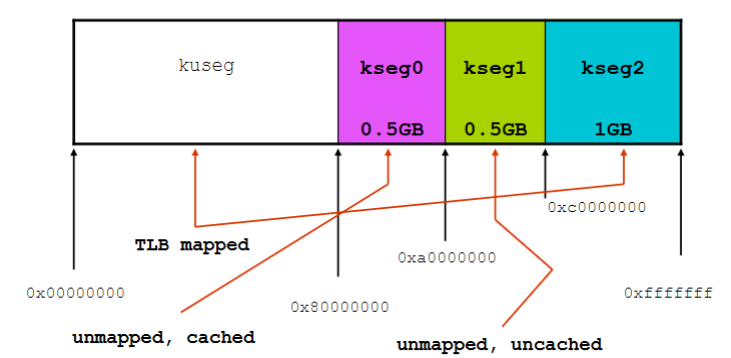
\includegraphics[width=\linewidth]{content/OS_Internals/images/2026-05-05-13-41-57.png}
  \end{minipage}
\end{center}






